\documentclass[8pt]{beamer}

\usepackage[utf8]{inputenc}
\usepackage{default}
\usepackage{hyperref}
\usepackage{textpos}
\usetheme{Copenhagen}

\title{Deep Learning}
\subtitle{Data encoding / representation}
\author{Tero Keski-Valkama}
\institute{\includegraphics[height=1.4cm]{CybercomG_logo_Classic_RGB.png}}
\date{2016-09-22}

\addtobeamertemplate{frametitle}{}{%
\begin{textblock*}{100mm}(10.95cm,-0.8cm)
\includegraphics[height=0.8cm]{cybercom-blue.png}
\end{textblock*}}


\begin{document}

\frame{\titlepage}
 
\begin{frame}
\frametitle{A quick recap}
\begin{itemize}
 \item Deep learning refers to deep neural networks. 1990s networks were shallow, and hence relatively useless.
 \item Neural networks are just complex non-linear models with lots of parameters. They are formed by layers of neurons, successive operations
       with an a linear combination of inputs from the previous layer and an activation function.
 \item In general, you always need a training set, a test set and a validation set. Training set is used to tune parameters, test set is used to tune hyperparameters,
       and validation set is used to check that the model does not overfit the test set. Boottrapping can be used to validate the data sectioning.
 \item Underfitting = high bias, overfitting = high variance
\end{itemize}

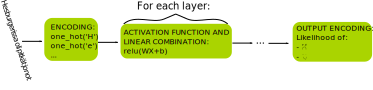
\includegraphics[width=0.9\textwidth]{./sentiment_analysis.png}

\end{frame}

\begin{frame}
\frametitle{Training Neural Networks}
\begin{itemize}
 \item In supervised training, the neural networks requires input and target output. The system finds a layered non-linear function from input to output.
 \item In unsupervised training, the network is only given input, and it learns a structure that captures the input statististical distributions and correlations.
 \item Unsupervised training uses energy-based methods which are better able to capture deep associations than a simple backpropagation, hence it is used for pre-training.
 \item A good platform to use for neural network experimentation is Google's TensorFlow, based on Python.
 \item Data representation is critical in neural networks, in the input representation, in the output representation (and by extension in defining the loss function), and
       also in the internal neuron representation.
\end{itemize}
\end{frame}

\begin{frame}
\frametitle{Tips \& Tricks}
 \begin{block}{Data Representation}
  \begin{itemize}
   \item Input representation
   \begin{itemize}
    \item Boolean values, Continuous values
    \item One-hot encoding for encoding exclusive choice
    \item Encoding time
   \end{itemize}
   \item Output representation
   \begin{itemize}
    \item Boolean values, Continuous values
    \item One-hot encoding for encoding exclusive choice
    \item Mixture distributions
   \end{itemize}
   \item Internal representation
   \begin{itemize}
    \item Abstraction levels
    \item Bottlenecks and compression
   \end{itemize}
  \end{itemize}
 \end{block}
\end{frame}

\begin{frame}
\frametitle{Input Representation}
 \begin{itemize}
  \item 
 \end{itemize}
\end{frame}

\begin{frame}
\frametitle{Output Representation / Categorical and Class Outputs}
 \begin{itemize}
  \item Categorical outputs refer to a situation where the output can take one out of a limited set of values. These are used for example in classification tasks where
        the input signal is classified to represent one of predetermined classes. For example ``cat'' vs. ``dog'', or ``walking'' vs. ``driving''.
  \item For categorical outputs, one-hot softmax encoding is typically used. In generation, the outputs represent probabilities for picking a specific category.
  \item Softmax normalizes the sum of the output values to be one, and scales all values to be positive, i.e. forms a proper probability distribution.
  \item The loss is calculated using cross entropy. In Tensorflow, you skip the softmax layer in the loss function and use the unnormalized outputs (interpreted as log-probabilities)
        directly with the tf.nn.softmax\_cross\_entropy\_with\_logits function.
  \item Sometimes the outputs are not mutually exclusive. For example, a photo might contain both a cat and a person. In these cases you normalize each output
        between 0 and 1 using a sigmoid function. In Tensorflow, you would use tf.nn.sigmoid\_cross\_entropy\_with\_logits function to calculate the loss from raw, unscaled outputs.
 \end{itemize}
\end{frame}

\begin{frame}
\frametitle{Output Representation / Mixture Density Outputs}
 \begin{itemize}
  \item For continuous values, it makes sense to use mixture density distributions, that is, using a weighted mixture of several distributions (e.g. 3 x normal distributions) with
        parameters (for normal distribution: means and variances) estimated by the network.
  \item The relative weights are softmaxed to represent a discrete probability distribution, much like categorical outputs above.
  \item The distribution parameters are normalized to an appropriate range if necessary, for example variance of the normal distribution
        is typically transformed through exp() function to
        limit it to be always non-negative. This also has a rationale from statistical likelihoods.
  \item Generating values from mixture density distributions is done by first picking the distribution index from the set of distributions using the relative weight probabilities.
  \item Then a value is picked from the selected distribution using sampling from that kind of distribution with those parameters.
  \item Mixture density distributions work especially well for continuous physical signals where the system has several different ``decisions''
        to make from moment to moment. This corresponds to degrees of freedom in some sense.
  \item It is not always clear how many distributions you should use. Analogous to K-means clustering.
 \end{itemize}
\end{frame}

\begin{frame}
\frametitle{Output Representation / Audio}
 \begin{itemize}
  \item In audio signals, it has been noted that instead of using mixture density distributions it is better to use one-hot softmax classes for different
        signal values at a certain time.
  \item This corresponds to a discrete distribution, and it works better because it is not clear for audio signals how many mixtures one should use.
  \item To keep the output tractable, the signal levels are squashed from full 16 bit to for example 255 different values using $\mu$ law encoding.
        \footnote{\href{https://deepmind.com/blog/wavenet-generative-model-raw-audio/}
                       {https://deepmind.com/blog/wavenet-generative-model-raw-audio/}}
 \end{itemize}
\end{frame}

\begin{frame}
\frametitle{Internal Representation}
 \begin{itemize}
  \item 
 \end{itemize}
\end{frame}

\begin{frame}
\frametitle{What did we learn?}
 \begin{itemize}
  \item To make neural networks learn effectively, the data must be represented in a suitable fashion.
 \end{itemize}
\end{frame}

\end{document}

